\part*{16.09.2014 - Amplificatori Operazionali Ideali}

\section{Introduzione}

In questa sessione di laboratorio abbiamo montato due circuiti con amplificatori operazionali: un generatore di corrente costante e un sommatore pesato. Nel primo caso abbiamo controllato se la corrente rimanesse costante al variare della resistenza di carico; nel secondo caso abbiamo valutato la tensione di uscita.

\section{Materiali}

\begin{itemize} [noitemsep]
\item Oscilloscopio Agilent DSO-X 2002A (bandwidth $70$ \si{\mega\hertz}, sample rate $2$ GSa/s);
\item Generatore di tensione continua Agilent E3631A (max $\pm 25$ \si{\volt} o $\pm 6$ \si{\volt});
\item Generatore di tensione Agilent 33120A con range di frequenza da $100$ \si{\micro\hertz} a $15$ \si{\mega\hertz};
\item Multimetro Agilent 34410A (utilizzato come amperometro e per verificare i valori delle resistenze);
\item Un amplificatore operazionale UA741;
\item Resistenze di vari valori;
\item Due capacità da $0.1$ \si{\micro\farad} (i valori misurati sono in Figura \ref{gr:costante});
\item Breadboard e cablaggi vari.
\end{itemize}

\section{Premessa sugli amplificatori operazionali ideali}

Durante l'esperienza valuteremo l'amplificatore operazionale considerandolo come ideale. Infatti, in questa approssimazione (peraltro non eccessivamente limitante visti i valori di corrente in gioco nel nostro caso), valgono (considerando come A e B rispettivamente gli ingressi invertente e non invertente):

\begin{equation}
\Delta V_{AB}=0
\label{eq:regola_V}
\end{equation}
\begin{equation}
I_{AB}=0
\label{eq:regola_I}
\end{equation}

cioè la ddp fra l'ingresso invertente e non invertente è portato ad essere nullo dall'amplificatore operazionale modificando il valore di tensione in output (il cosiddetto \textit{ground virtuale} dato che nei nostri casi l'ingresso non invertente è collegato alla comune del circuito); e la corrente assorbita dall'amplificatore è nulla.
Queste regole verranno utilizzate durante questa sessione per valutare la risposta del circuito a segnali in ingresso, e si intendono utilizzate per tutte le sessioni in cui l'amplificatore è considerato ideale.

\begin{figure}[ht]
 \centering
   {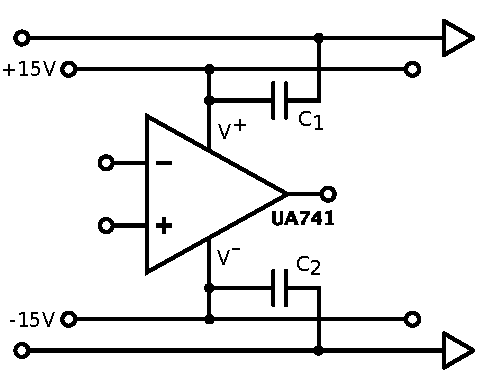
\includegraphics[width=6cm]{../E01/latex/alimentazione.pdf}}
 \caption{Grafico dell'alimentazione dell'OPAMP. La tensione di alimentazione è fornita con il generatore di tensione costante, mentre le capacità sono $C_1=(0.112 \pm 0.001)$ \si{\micro\farad} $C_2=(0.095\pm0.001)$ \si{\micro\farad}. Per maggiore chiarezza negli schemi circuitali, questa configurazione sarà nascosta negli schemi successivi, ma comunque presente sulla breadboard.}
 \label{gr:costante}
\end{figure}

Inoltre, al fine di evitare problemi di rumore durante l'alimentazione, abbiamo collegato l'alimentazione a due capacità come nello schema in Figura \ref{gr:costante}.

\section{Generatore di corrente}

In questo circuito abbiamo assemblato un generatore di corrente costante, cioè un dispositivo in grado di erogare una corrente costante ai capi di una resistenza (che definiremo \textit{resistenza di carico} $R_c$), indipendentemente dal valore di quest'ultima. Per valutare questa caratteristica abbiamo dunque utilizzato come $R_c=R_2$ una resistenza variabile di tipo \textit{trimmer}. Lo schema circuitale è in Figura \ref{gen_continua}.

\begin{wrapfigure}[21]{r}{0.55\textwidth}
  \begin{center}
    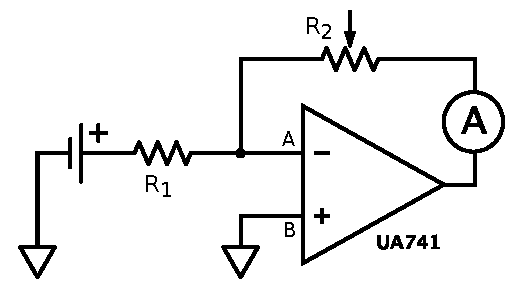
\includegraphics[width=0.40\textwidth]{../E01/latex/c1.pdf}
  \end{center}
  \caption{Schema del generatore di corrente costante. Come valori abbiamo utilizzato $R1=(3.85 \pm 0.01)$ \si{\kilo\ohm} e $V_{gen}=3.85$ \si{\volt}, mentre $R_2$ è variabile. Come amperometro è utilizzato il multimetro, mentre per alimentare l'OPAMP e come generatore di tensione costante in figura, abbiamo utillizzato il generatore Agilent E3631A.}
  \label{gen_continua}
\end{wrapfigure}

Risolviamo ora il circuito, considerando la tensione fornita dal generatore di tensione continua come $V_{gen}$ e la tensione in uscita dall'OPAMP come $V_{out}$. Dato che B si trova a potenziale di comune, per (\ref{eq:regola_V}) anche A sarà allo stesso potenziale, che considereremo nullo. Dunque varranno
\begin{equation}
V_{gen} - V_A = V_{gen} = I_1 R_1
\label{eq:gen_1}
\end{equation}
$$V_{out} - V_A = V_{out} = I_2 R_2$$
Per (\ref{eq:regola_I}) e la legge di Kirkhhoff sui nodi, avremo invece che la corrente passante per la resistenza di carico è uguale alla corrente di (\ref{eq:gen_1}) in modulo e varrà: $I=I_1=-I_2$.

Otteniamo dunque che la tensione di output si modificherà, ad opera dell'OPAMP, in modo da far passare sempre lo stesso valore di corrente attraverso $R_2$; ciò avviene per il fenomeno di retroazione negativa, che ci permette di controllare la tensione di output tramite la resistenza di feedback, che in questo caso è $R_2$, e di ottenere dunque una corrente costante passante per il circuito di feedback. Imponendo l'uguaglianza della corrente possiamo inoltre trovare il valore della tensione di uscita

$$V_{out}=-\frac{R_2}{R_1} V_{gen}$$

Durante l'esperienza abbiamo però deciso di misurare la corrente passante per la resistenza piuttosto che la tensione di uscita, ponendo un amperometro fra l'uscita dell'OPAMP e la resistenza di carico $R_2$. Come valore di corrente abbiamo scelto $1$ \si{\milli\ampere}, discostandoci dalla corrente massima in cui l'amplificatore operazionale potrebbe non comportarsi più in maniera ideale ($10/20$ \si{\milli\ampere}); e avendo a disposizione una resistenza $R_1=(3.85 \pm 0.01)$ \si{\kilo\ohm}, per (\ref{eq:gen_1}), abbiamo utilizzato una tensione continua di $3.85$ \si{\volt}. Di seguito proponiamo alcuni valori sperimentali che confermano la capacità del circuito da noi creato di fornire alla resistenza di carico una corrente costante di $1$ \si{\milli\ampere}.

\begin{center}
\begin{tabular}{c|c|c|c|c|c|c|c|c}
Resistenza variabile [\si{\ohm}] & 0.54 & 35.1 & 412 & 1021 & 1996 & 3068 & 4170 & 4719 \\ 
\hline 
Corrente nel carico [\si{\milli\ampere}] & 1.002 & 1.002 & 1.002 & 1.002 & 1.002 & 1.002 & 1.002 & 1.002 \\ 
\end{tabular}
\end{center}

Gli errori sulla tabella sono uguali, cioè unitari sull'ultima cifra del valore, sia per le resistenza che per le correnti.

\section{Sommatore Pesato}

\subsection{Circuito}

Valutiamo ora il sommatore pesato, cioè un circuito che dati alcuni segnali in ingresso (due nel nostro caso) li somma con relativi pesi dati dal rapporto fra la resistenza di feedback ($R_f$) e quella a loro associata ($R_1$ e $R_2$). Lo schema circuitale è in Figura \ref{sommatore_pesato}.

\begin{wrapfigure}[21]{l}{0.55\textwidth}
  \begin{center}
    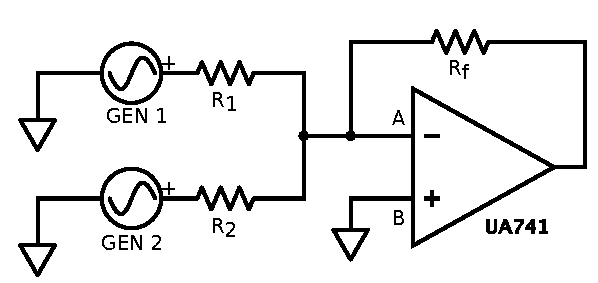
\includegraphics[width=0.40\textwidth]{../E01/latex/c2.pdf}
  \end{center}
  \caption{Schema del sommatore pesato. Come valori abbiamo utilizzato $R_f=(99.7 \pm 0.1)$ \si{\kilo\ohm}, $R_1=(99.9 \pm 0.1)$ \si{\kilo\ohm} e $R_2=(49.8 \pm 0.1)$ \si{\kilo\ohm}, dove per $R_2$ è stato necessario utilizzare un parallelo di due resistenza da $100$ \si{\kilo\ohm}. Come GEN 1 abbiamo utilizzato l'oscilloscopio, mentre per GEN 2 il generatore di forme d'onda. Infine, per valutare la tensione in uscita abbiamo utilizzato l'oscilloscopio.}
  \label{sommatore_pesato}
\end{wrapfigure}

Per risolvere il circuito consideriamo, definendo le tensioni dei generatori 1 e 2 rispettivamente $V_1$ e $V_2$, le seguenti equazioni derivanti dalle leggi di Kirkhhoff e dalla (\ref{eq:regola_I})
$$V_1 - V_A =I_1 R_1 \qquad V_2 - V_A =I_2 R_2$$
$$V_A - V_{out} =(I_1+I_2) R_f$$
Per (\ref{eq:regola_V}) vale inoltre che $V_A=V_B=0$; dunque otteniamo, sostituendo le correnti nell'ultima equazione sopra
$$V_{out}=-R_f \left( \frac{V_1}{R_1}+\frac{V_2}{R_2}\right)$$

Si può dunque definire un peso relativo $\phi_i$ ad ogni segnale dato dal rapporto fra $R_f$ ed $R_{i}$ (con $i=1,2$) e scrivere una formula del tipo
$$V_{out}=-\sum^{2}_{i=1} \frac{R_f}{R_{i}}V_{i}=-\sum^{2}_{i=1} \phi_i V_{i}$$

Durante l'esperienza abbiamo optato per valori semplici dei rapporti fra le resistenze, utilizzando i seguenti valori: $R_f=R_1=100 k\Omega$ e $R_2=50 k\Omega$. Si ottengono dunque $\phi_1=1$ e $\phi_2=2$.

\subsection{Grafici}

Presentiamo ora i grafici di alcune forme d'onda in uscita.

$$$$

\begin{figure}[ht]
 \centering
   {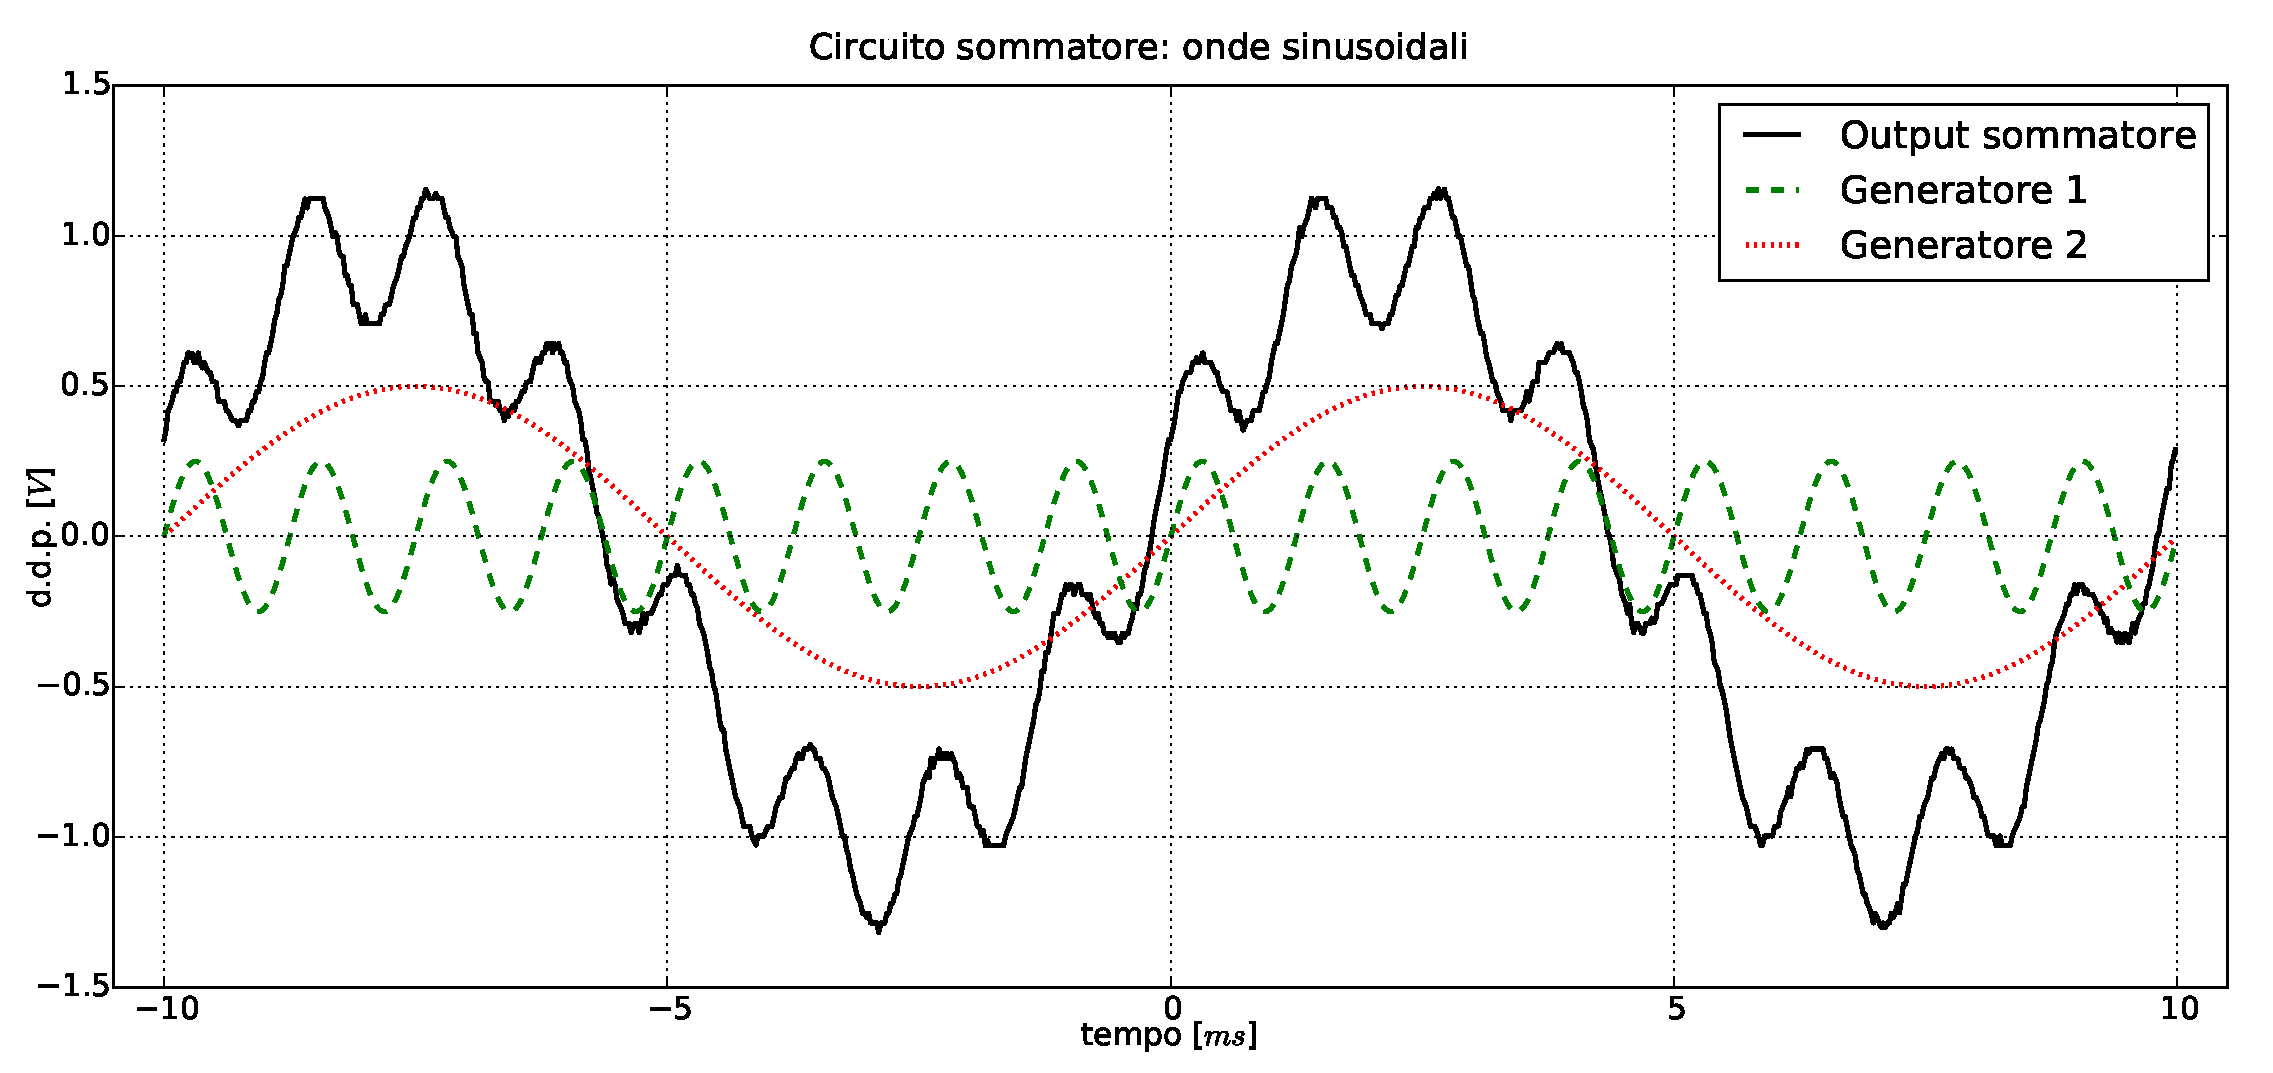
\includegraphics[width=16.5cm]{../E01/latex/sinsin.pdf}}
 \caption{Grafico della tensione di uscita. Il generatore 1 (generatore dell'oscilloscopio) crea un'onda sinusoidale di $\nu=800$ \si{\hertz} e $V^1_{pp}=500$ \si{\milli\volt}; il generatore 2 (generatore di forme d'onda) crea invece un'onda sinusoidale di $\nu=100$ \si{\hertz} e $V^2_{pp}=1000$ \si{\milli\volt}. Notiamo inoltre che l'ampiezza massima è pari a $\phi_1 V^1_{pp}+\phi_2 V^2_{pp}=2500$ \si{\milli\volt}.}
 \label{gr:onde1}
\end{figure}

$$$$

\begin{figure}[ht]
 \centering
   {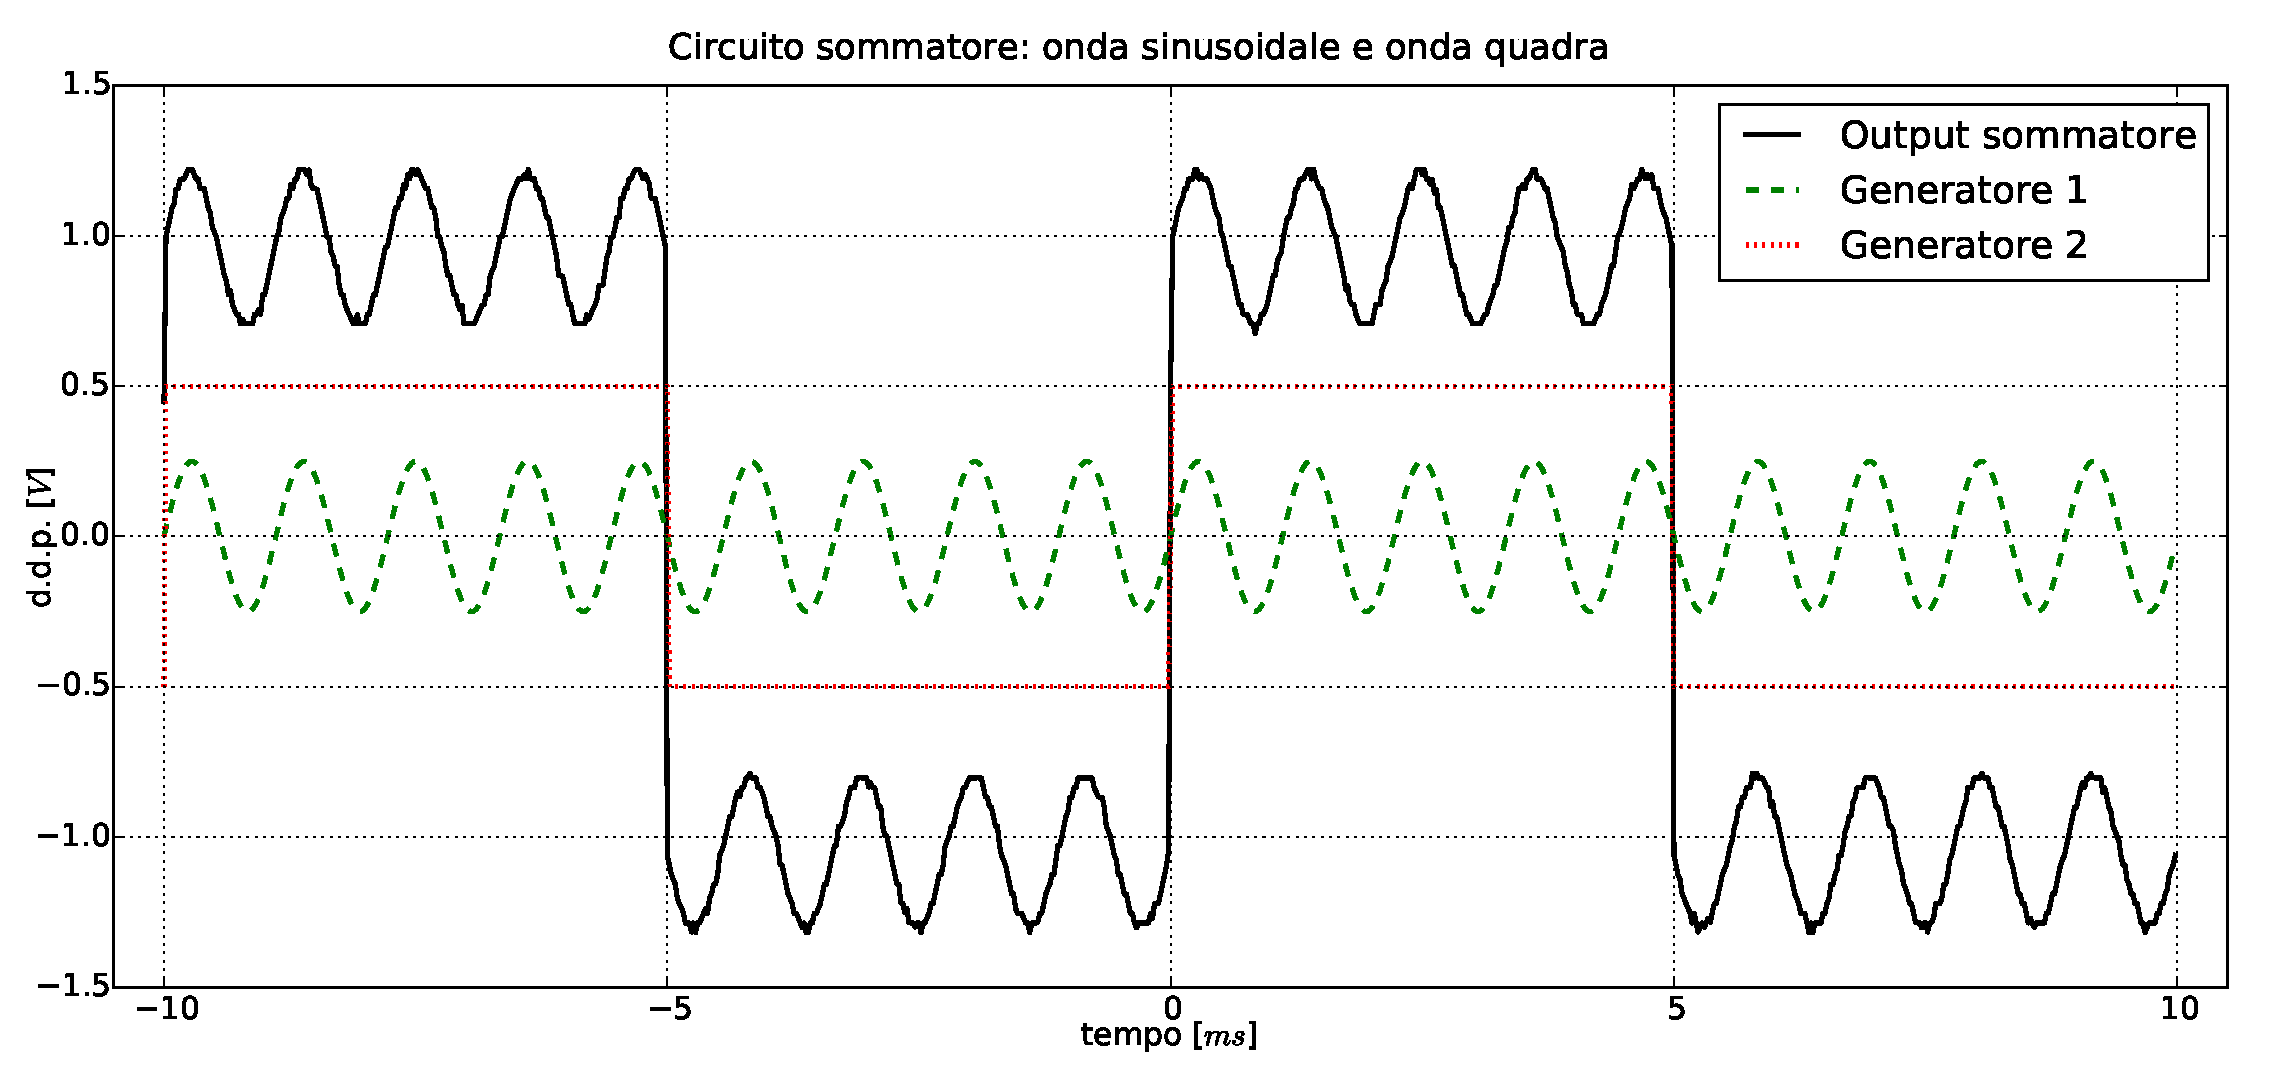
\includegraphics[width=16.5cm]{../E01/latex/sinquad.pdf}}
 \caption{Grafico della tensione di uscita. Il generatore 1 (generatore dell'oscilloscopio) crea un'onda sinusoidale di $\nu=900$ \si{\hertz} e $V^1_{pp}=500$ \si{\milli\volt}; il generatore 2 (generatore di forme d'onda) crea invece un'onda quadra di $\nu=100$ \si{\hertz} e $V^2_{pp}=1000$ \si{\milli\volt}. Notiamo inoltre che anche in questo caso l'ampiezza massima è pari a $\phi_1 V^1_{pp}+\phi_2 V^2_{pp}=2500$ \si{\milli\volt}.}
 \label{gr:onde2}
\end{figure}

\subsection{Battimenti}

Utilizzando due forme d'onda sinusoidali con il sommatore, abbiamo potuto il battimento, fenomeno che si verifica quando la differenza fra le frequenze delle onde in ingresso è sufficientemente bassa.

Con due onde abbiamo che:
\begin{equation}
V_{out}=\phi_1 A_1 \sin [2 \pi \nu_1 t + \theta_1] + \phi_2 A_2 \sin [2 \pi \nu_2 t + \theta_2]
\label{eq: battimenti1}
\end{equation}

Supponiamo che $A=\phi_1 A_1=\phi_2 A_2$, come nel caso del grafico sotto riportato, in modo da poter applicare le formule di prostaferesi. Otteniamo che

$$V_{out}=2A \cos \left[\pi (\nu_1 - \nu_2)t + \frac{\theta_1-\theta_2}{2}\right] \sin \left[\pi (\nu_1 + \nu_2) t + \frac{\theta_1+\theta_2}{2}\right]$$

Dunque, se consideriamo $\nu_1 + \nu_2 >> |\nu_1 - \nu_2|$, otteniamo il battimento. Notiamo inoltre che, nel grafico in Figura \ref{gr:onde1} (caso in cui non vale la condizione sopra), non si osserva il fenomeno del battimento.

\begin{figure}[ht]
 \centering
   {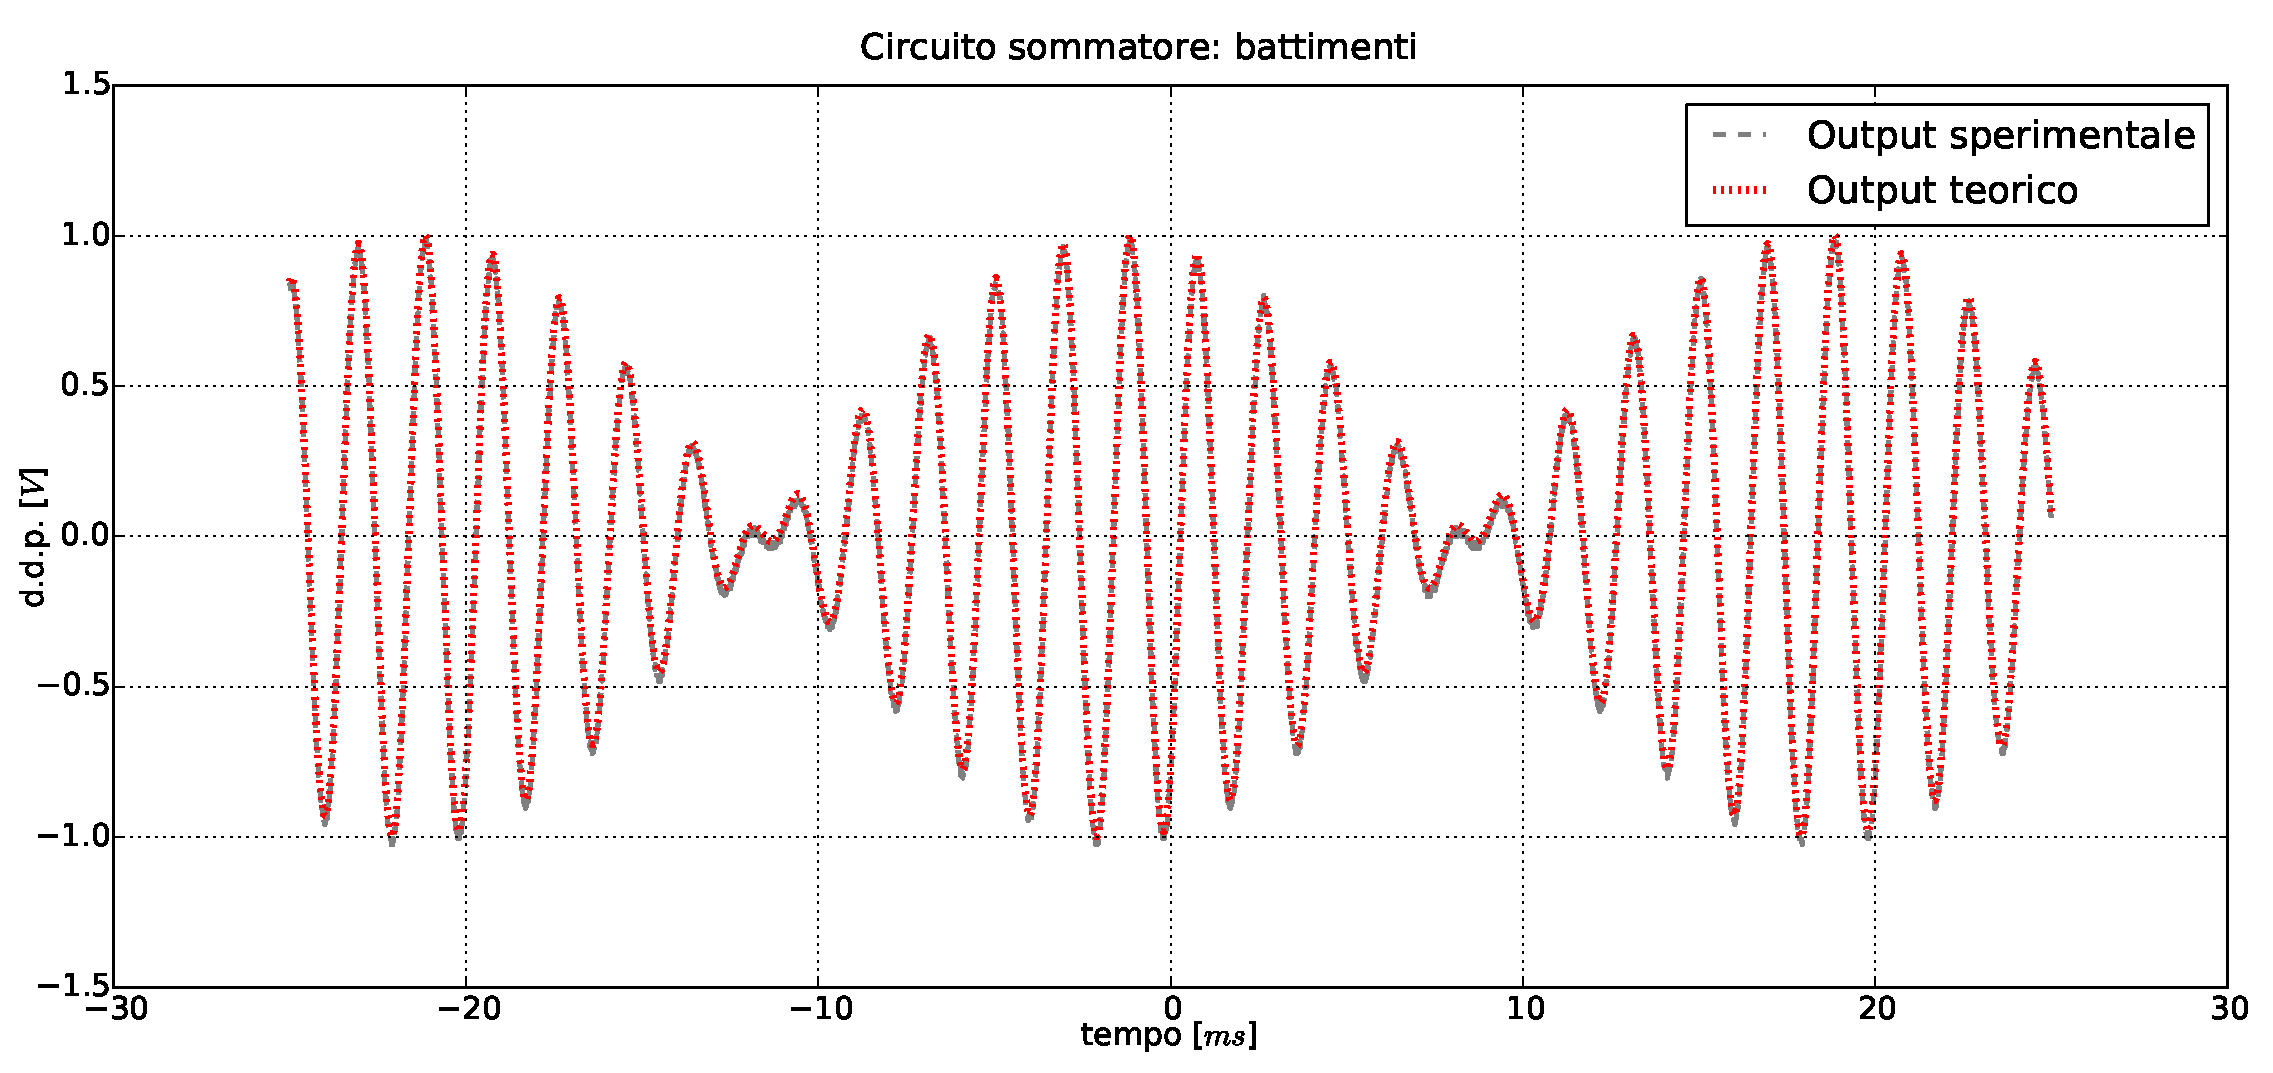
\includegraphics[width=17.5cm]{../E01/latex/battimenti_ideali.pdf}}
 \caption{Grafico della tensione di uscita. Il generatore 1 (generatore dell'oscilloscopio) crea un'onda sinusoidale di $\nu=550$ \si{\hertz} e $V^1_{pp}=1000$ \si{\milli\volt}; il generatore 2 (generatore di forme d'onda) crea invece un'onda quadra di $\nu=500$ \si{\hertz} e $V^2_{pp}=250$ \si{\milli\volt}. Notiamo inoltre che l'ampiezza massima è data da $A = 2 \phi_1 A_1 = 2 \phi_2 A_2 = 1000$ \si{\milli\volt}, coerentemente con la teoria sopra esposta. L'output teorico è stato valutato con un fit sulla legge (\ref{eq: battimenti1}).}
 \label{gr:battimenti}
\end{figure}